
\documentclass[11pt]{article}

\usepackage{fullpage,epsfig,latexsym,picinpar,amsbsy,amsmath,algorithm}
\usepackage[noend]{algpseudocode}
\usepackage{xspace}


\setlength{\evensidemargin}{0.1in}
\setlength{\oddsidemargin}{0.1in}
\setlength{\textwidth}{6.6in}
\setlength{\topmargin}{0.0in}
\setlength{\textheight}{8.7in}
\setlength{\headheight}{0in}
\setlength{\headsep}{0in}
\setlength{\topsep}{0in}
\setlength{\itemsep}{0in}
\renewcommand{\baselinestretch}{1.1}
\parskip=0.080in
                                                                                                                         
\newcommand{\parend}[1]{{\left( #1  \right) }}
\newcommand{\spparend}[1]{{\left(\, #1  \,\right) }}
\newcommand{\angled}[1]{{\left\langle #1  \right\rangle }}
\newcommand{\brackd}[1]{{\left[ #1  \right] }}
\newcommand{\spbrackd}[1]{{\left[\, #1  \,\right] }}
\newcommand{\braced}[1]{{\left\{ #1  \right\} }}
\newcommand{\leftbraced}[1]{{\left\{ #1  \right. }}
\newcommand{\floor}[1]{{\left\lfloor #1\right\rfloor}}
\newcommand{\ceiling}[1]{{\left\lceil #1\right\rceil}}
\newcommand{\barred}[1]{{\left|#1\right|}}
\newcommand{\doublebarred}[1]{{\left|\left|#1\right|\right|}}
\newcommand{\spaced}[1]{{\, #1\, }}
\newcommand{\suchthat}{{\spaced{|}}}
\newcommand{\numof}{{\sharp}}
\newcommand{\assign}{{\,\leftarrow\,}}
                                                                                                                         
\newcommand{\veps}{{\varepsilon}}
\newcommand{\Sigmastar}{{\Sigma^\ast}}
\newcommand{\barx}{{ \bar x}}

\newcommand{\half}{{\mbox{$\frac{1}{2}$}}}
\newcommand{\threehalfs}{{\mbox{$\frac{3}{2}$}}}





\usepackage{listings}
\usepackage{color}

\definecolor{dkgreen}{rgb}{0,0.6,0}
\definecolor{gray}{rgb}{0.5,0.5,0.5}
\definecolor{mauve}{rgb}{0.58,0,0.82}

\lstset{frame=tb,
  language=Java,
  aboveskip=3mm,
  belowskip=3mm,
  showstringspaces=false,
  columns=flexible,
  basicstyle={\small\ttfamily},
  numbers=none,
  numberstyle=\tiny\color{gray},
  keywordstyle=\color{blue},
  commentstyle=\color{dkgreen},
  stringstyle=\color{mauve},
  breaklines=true,
  breakatwhitespace=true,
  tabsize=3
}

\begin{document}

\centerline{\large \bf CS235 ASSIGNMENT}
\centerline{Yidi Wang}
\centerline{862114701}

\vskip 0.1in

%%%%%%%%%%%%%%%%%%%%%%%%%%%%

\paragraph{Question 1}\mbox{} \\
\noindent
\textbf{Part 1}
\begin{verbatim}
clear; clc;
edgelist = dlmread('graph.txt');
edgelist = unique(edgelist, 'rows');
A = sparse(edgelist(:,1), edgelist(:,2), 1);
\end{verbatim}

\noindent
\textbf{Part 2, 3} \\
There are mainly two dense blocks are annotated by red circles.
\begin{figure}[H]
    \centering
    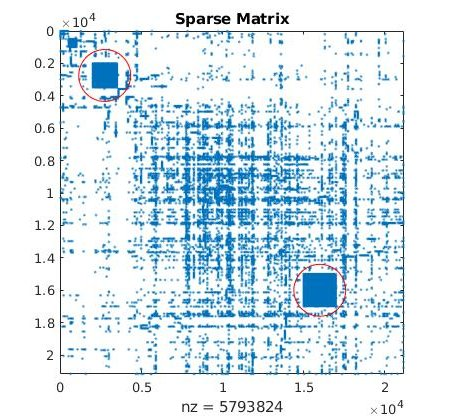
\includegraphics[scale=0.56]{figs/q1.jpg}
    \caption{spy-plot}
    \label{fig::spy}
\end{figure}

%%%%%%%%%%%%%%%%%%%%%%%%%%%%
\paragraph{Question 2}\mbox{} \\
\noindent
\textbf{Part 1} \\
The number of connected nodes are calculated for each node in the edge-list of the graph.
\begin{verbatim}
max_node = max(edgelist(:));
deg_node = zeros(1, max_node);
for i = 1:max_node
    deg_node(i) = sum(rows(:) == i);
end
\end{verbatim}

\noindent
\textbf{Part 2} \\
\begin{figure}[H]
    \centering
    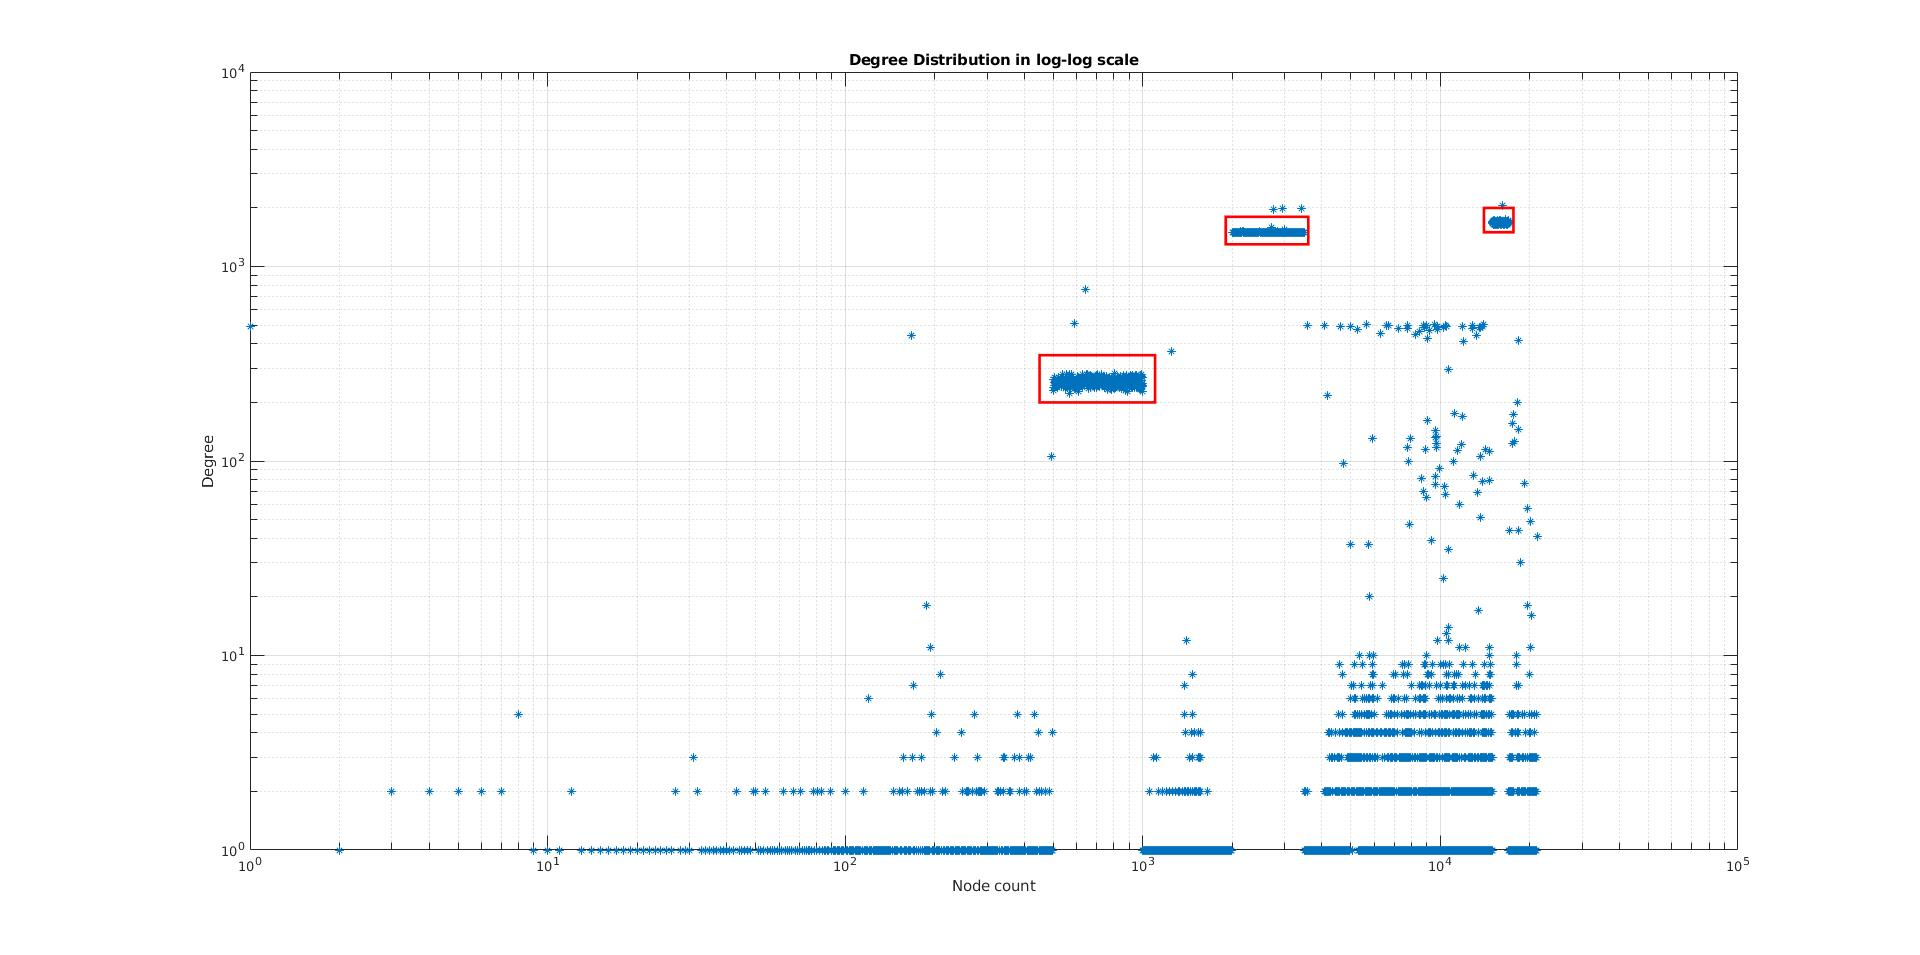
\includegraphics[width=\linewidth]{figs/q2.jpg}
    \caption{Degree distribution in log-log scale}
    \label{fig::deg_log}
\end{figure}

\noindent
\textbf{Part 3} \\
Yes. In the clean degree distribution figure, the majority of the nodes have a small degree. While the degree becomes larger, the number of corresponding nodes become less and less. Degree and node counts are negtively correlated. However, in this distribution, node count is increasing while the degree increase. They are positively correlated.

\noindent
\textbf{Part 4} \\
(a). There are mainly twoe abnormal blocks. They are annotated in red circles. Above the $10^2$ on the y axis in the above figure (when degree is big enough), there are two (near-)horizontal lines, which means that there are many consecutive nodes having similar degrees. This will cause dense blocks in the sparse matrix.c \\
\noindent
(b). The lower left thick line in Fig.\ref{fig::deg_log} is corresponding to the lowest right dense block in Fig.\ref{fig::spy}. And the upper right thick line in Fig.\ref{fig::deg_log} is corresponding to the upper left block in Fig.\ref{fig::spy}.

\paragraph{Question 3}\mbox{} \\
\noindent
\textbf{Part 1} \\
\noindent
Main Problem \newline
The goal of this paper is to extract community-like structures rather than graph-partitioning. The traditional methods, spectral clustering and multi-level graph partitioning can not yield good communities in the graph.

\noindent
Main Idea \newline
They use undirected graphs, which is represented as a adjacant matrix. The matrix is square and symmetric. In such a matrix, the eigenvalues are non-zero and the singular vectors coincide with the non-null eigenvectors. To use the features in their research, they expect to see communities in the form of (near-)cliques or (near-)bi-partite cores among the nodes in the spokes. From the EE-plot, they found that the linear nature of spokes means that the scores of the nodes are linear correcletd; therefore, exploring dominant nodes along one singular vector should be sufficient to extract nodes of a community.

\noindent
Results \newline
They use SpokEn to extract the communities in four Mobile Call graphs, which shows that SpokEn has successfully stopped at the termination criterion. Then they tested SpokEn with some real world graphs. Some typical results are given in figure 6. A bipartite from patent graph, a clique and a bipartite from provider-customers show that SpokEn works well.

\noindent
\textbf{Part 2} \\
(a). % TODO: compute square error
\begin{verbatim}
[u,s,v] = svds(A);
ds = diag(s);
dsp = norm(ds(n+1:end)) / norm(ds);
\end{verbatim}
I tried the above code with different $n$. When $n = 2$, the error is $0.1157$. When $n = 3$, the error is $0.0271$. So, if we want a reconstruction correctness larger than $90\%$, the number of singular value is 3.
$$
\begin{bmatrix} 
    1679.9  \\
    1501.0  \\ 
    255.22  \\
    37.715  \\
    35.5439
\end{bmatrix}
$$

\noindent
(b). 
\begin{figure}[H]
    \centering
    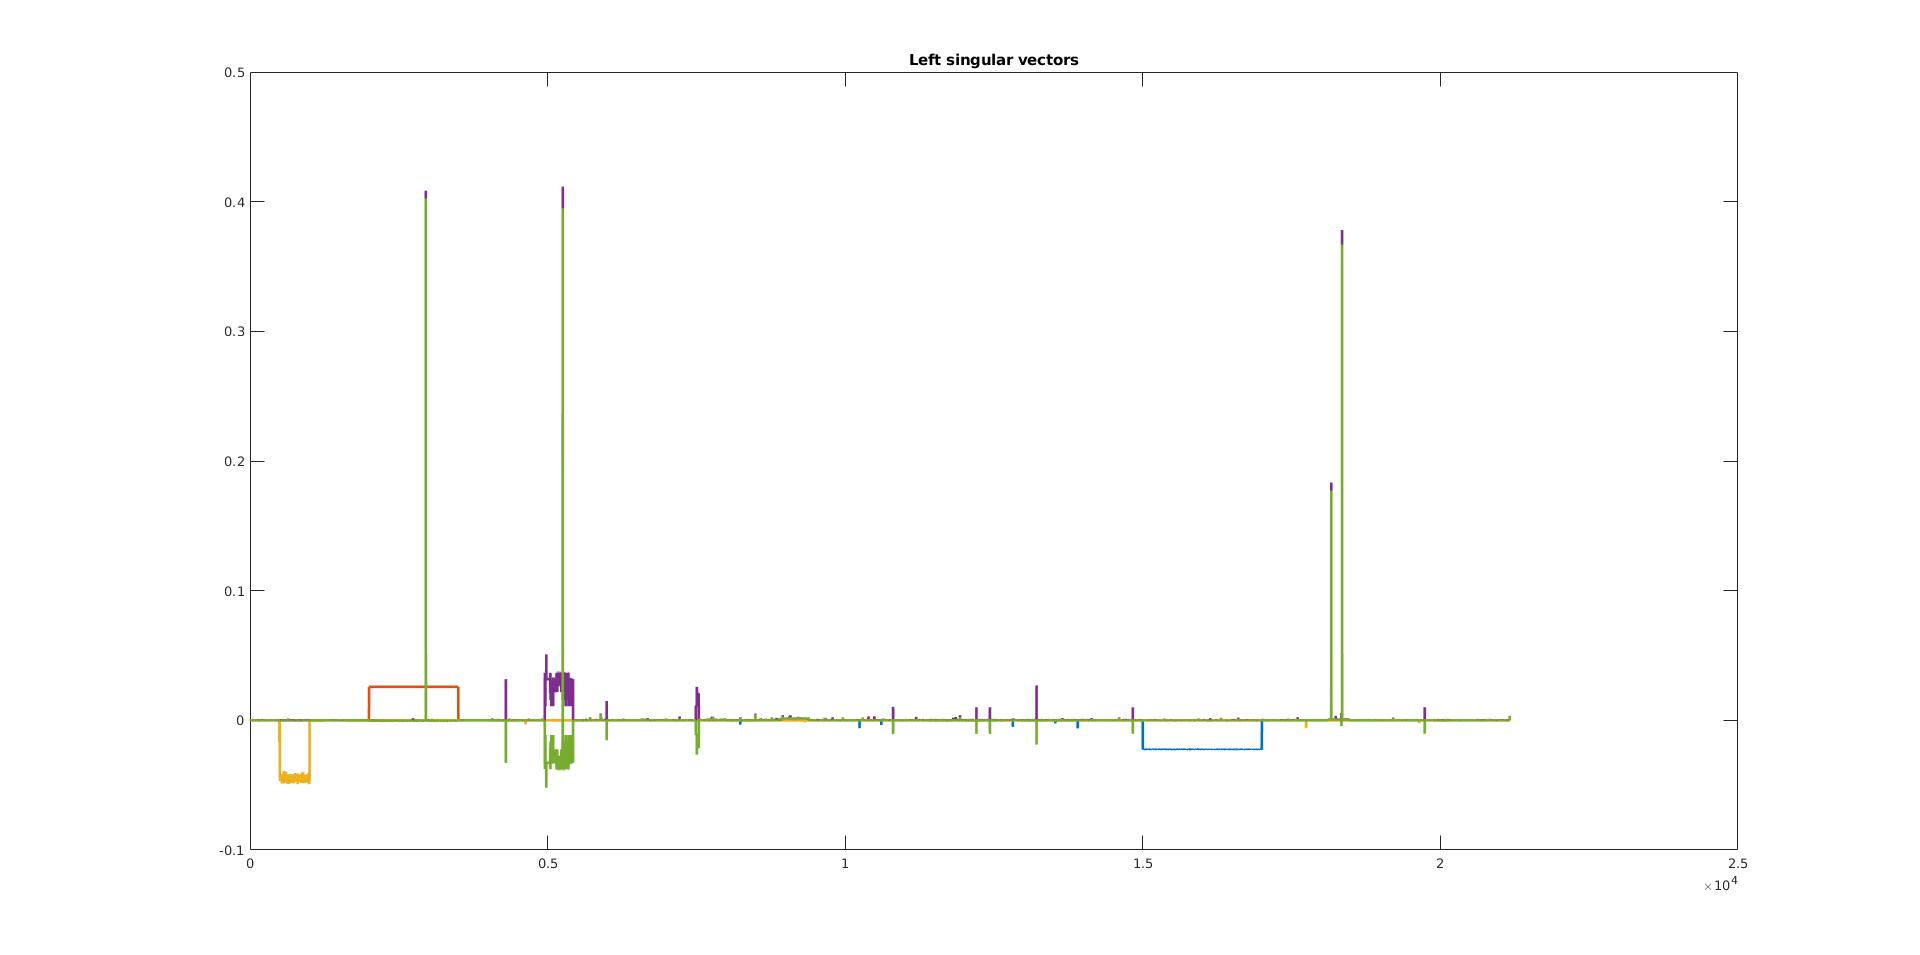
\includegraphics[width=\linewidth]{figs/q3.jpg}
    \caption{Left singular vectors}
    \label{fig::vec}
\end{figure}

\noindent
(c).
Any abnormal block in the spy-plot is a (near-)clique or a (near-)bipartite in the graph. In the paper, they proved that when they increase the number of communities, the spoke pattern on the EE-plot will become more clear. In the abpve left singular value plot, we have two long spokes, which are corresponding to the two dense blocks in the spy-plot in \ref{fig::spy}.

\noindent
(d).
\begin{figure}[H]
    \centering
    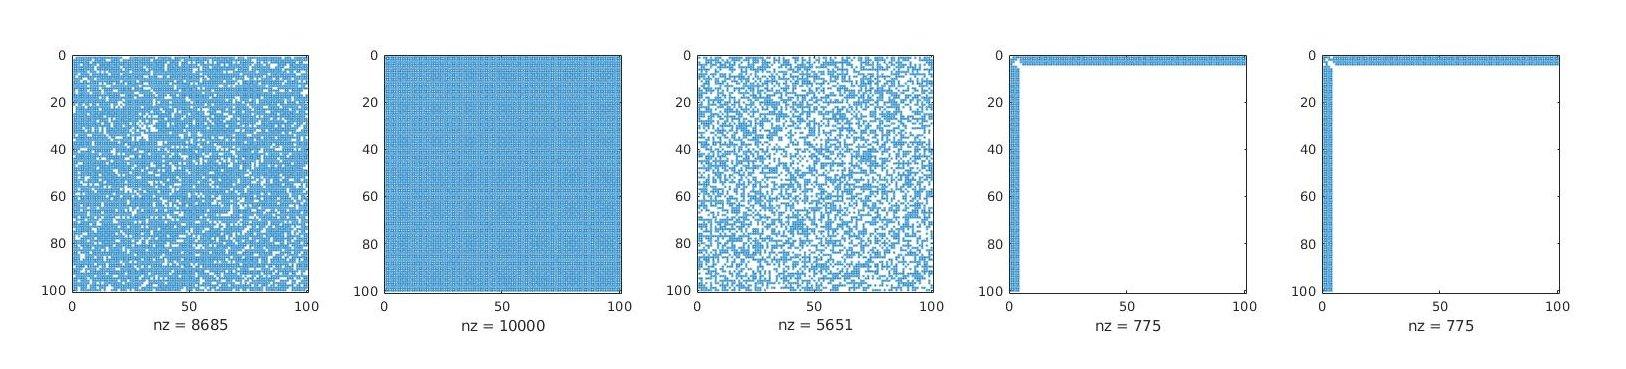
\includegraphics[width=\linewidth]{figs/q3_d.jpg}
    \caption{Left singular vectors}
    \label{fig::sub}
\end{figure}


\end{document}

